\section{Formal Structure of the Recursive Action}
\label{sec:recursive-action-formal}

\subsection{13.1 Recursive Action Definition}

The total action across cosmological cycles is defined as a sum over discrete recursive epochs:
\begin{equation}
\mathcal{A}_{\text{total}} = \sum_{n} \mathcal{A}_n
\end{equation}
Each term \( \mathcal{A}_n \) is the action functional for the \( n \)-th cycle, defined over the recursive configuration space \( \phi_n \in \mathcal{C}_n = (a_n, \varphi_n, \lambda_n, E_n) \), where:
\begin{itemize}
    \item \( a_n \): scale factor,
    \item \( \varphi_n \): scalar (matter) field configuration,
    \item \( \lambda_n \): coherence fidelity, \( \lambda_n = |\langle \Psi_{n-1} | \Psi_n \rangle|^2 \),
    \item \( E_n \): ER bridge entanglement eigenvalue.
\end{itemize}

The action per cycle decomposes into four sectoral contributions:
\begin{equation}
\mathcal{A}_n = \int d^4x \left[
\mathcal{L}_{\text{LQC}}(a_n, \varphi_n) +
\mathcal{L}_{\text{mem}}(\lambda_n) +
\mathcal{L}_{\text{ERB}}(E_n) +
\mathcal{L}_{\text{obs}}(\phi_n)
\right]
\end{equation}

\subsection{13.2 Components of the Recursive Action}

\paragraph{LQC Dynamics:}
\[
\mathcal{L}_{\text{LQC}} = \frac{1}{2} G^{IJ}(q) \dot{q}_I \dot{q}_J - V(q)
\]
where \( q = (a, \varphi) \) and \( G^{IJ} \) is the LQC field-space metric.

\paragraph{Memory Coupling Term:}
\[
\mathcal{L}_{\text{mem}} = -\beta^{-1} \log \lambda_n
\]
This penalizes coherence loss, modulated by the inverse memory temperature \( \beta^{-1} \).

\paragraph{Bridge Contribution:}
\[
\mathcal{L}_{\text{ERB}} = \frac{A(\phi_n, \phi_{n-1})}{4G} + i\lambda_E I(\phi_n, \phi_{n-1})
\]
where:
\[
I(\phi_n, \phi_{n-1}) := \mathrm{Tr}[\rho_n (\log \rho_n - \log \rho_{n-1})]
\]
quantifies quantum information divergence across the ERB. The term \( \lambda_E \) weights the coherence-entropy tradeoff.

\paragraph{Observer Projection Term:}
\[
\mathcal{L}_{\text{obs}} = \langle \Psi_n | \hat{O}_n | \Psi_n \rangle
\]
This captures effective decoherence via projection onto an observer subspace. \( \hat{O}_n \) is an external boundary condition operator (see Appendix~C.6.3).

\subsection{13.3 Symmetries and Variational Constraints}

Recursive symmetry requires:
\[
\Psi_n(\phi) \leftrightarrow \Psi_{-n}(\phi)
\]
under time reflection, assuming conformal invariance and minimal decoherence. Bounce structure remains symmetric in the semiclassical limit.

We impose:
- A **geometric entropy bound**:
\[
A(\phi_n, \phi_{n-1}) \geq \ell_{\text{Pl}}^2,
\]
- And a **variational coherence constraint**:
\[
\delta \mathcal{A}_n + \lambda_C \, \delta\left( S[\rho_n] - \lambda_S \log \lambda_n \right) = 0
\]
This enforces entropy–fidelity equilibrium, with \( \lambda_C \) acting as a coherence balance multiplier.

\subsection{13.4 Euler–Lagrange Equations}

Functional variation of the total action yields recursive field equations:

\paragraph{(1) Geometry (Scale Factor):}
\[
\ddot{a}_n + \frac{\partial V}{\partial a_n} + \frac{\partial \mathcal{L}_{\text{ERB}}}{\partial a_n} = 0
\]

\paragraph{(2) Scalar Field:}
\[
\ddot{\varphi}_n + \frac{\partial V}{\partial \varphi_n} + \frac{\partial \mathcal{L}_{\text{ERB}}}{\partial \varphi_n} = 0
\]

\paragraph{(3) Entanglement Eigenvalue (Coherence Field):}
Assuming:
\[
S(\rho_n \| \rho_{n-1}) \sim (E_n - E_{n-1})^2,
\]
define:
\[
V_E(E_n) := -S(\rho_n \| \rho_{n-1})
\quad \Rightarrow \quad
\ddot{E}_n + \lambda_E^{-1} \frac{\partial V_E}{\partial E_n} = 0
\]

\paragraph{(4) Memory Fidelity \( \lambda_n \):}
Treated as a constrained observable:
\[
\frac{\delta S[\rho_n]}{\delta \lambda_n} = \frac{\lambda_S}{\lambda_n}
\]

\paragraph{(5) Observer Projection:}
\[
\hat{O}_n \text{ fixed unless relational decoherence is modeled explicitly}
\]

These equations govern recursive attractor stability under entropy, memory, and boundary constraints.

\subsection{13.5 Interpretation}

This recursive action formalism integrates gravitational dynamics, coherence evolution, and observer-induced entropy into a unified variational structure. The universe is modeled not as a system evolving freely through spacetime, but as a signal constrained to remember — favoring configurations that maximize coherence while minimizing informational tension.

\textbf{Conclusion:} The recursive action functions as a memory-penalized path integral: the universe does not merely repeat — it filters. Only those paths that sustain coherence survive recursive evolution.

\begin{figure}[H]
\centering
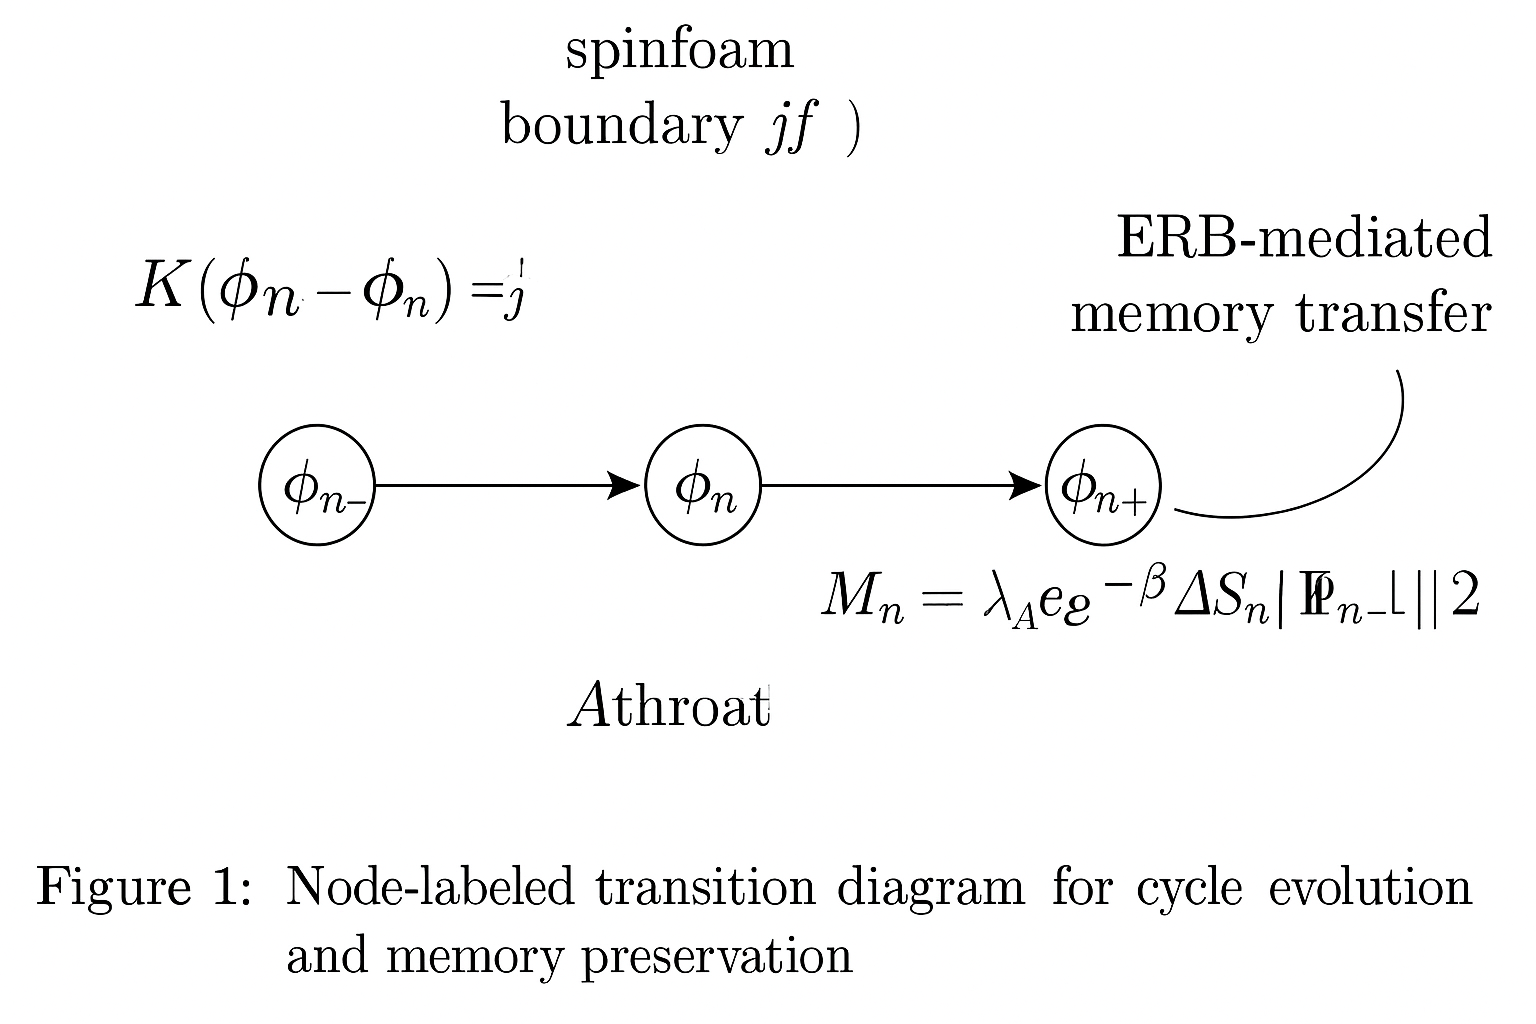
\includegraphics[width=0.75\textwidth]{figures/recursive_action_layers.png}
\caption{Layered structure of the recursive action. Each cycle contributes LQC dynamics, memory coupling, ER bridge entropy terms, and observer projection constraints. Recursive stability is governed by coherence feedback between cycles.}
\label{fig:recursive-action-layers}
\end{figure}
